\documentclass[a4paper,journal]{IEEEtran}
%\documentclass[conference]{IEEEtran}
%for using the therefore symbol
%\usepackage{amssymb}
%end

\usepackage[utf8]{inputenc}
\usepackage{graphicx}
\usepackage{float}
\usepackage{color, colortbl}
\usepackage{xcolor}
\usepackage{array}
\usepackage{multirow}
\usepackage{footnote}
\usepackage{cite}
%The below is used to add notes to tables without disrupting the IEEEtran format
\usepackage{threeparttable}
%Multiple figures in a row
%\usepackage{caption}
%\usepackage{subcaption}
\usepackage{amsmath}

% Disable below if wanting to comply exclusively to conference mode of IEEEtran
% \IEEEoverridecommandlockouts


\usepackage{lipsum}

\begin{document}
%opening
 \title{The Evolution of MAC for Wireless LANs}


%A more simple output, useful when involving people from different affiliations
  %\author{
    %  \IEEEauthorblockN{Luis Sanabria-Russo\IEEEauthorrefmark{0}, Jaume Barcelo\IEEEauthorrefmark{0}, Boris Bellalta\IEEEauthorrefmark{0}}\\
      %\IEEEauthorblockA{\IEEEauthorrefmark{0}Universitat Pompeu Fabra, Barcelona, Spain
      %\\\{luis.sanabria, jaume.barcelo, boris.bellalta\}@upf.edu}
  %}

\author{Luis Sanabria-Russo \\
		NeTS Research Group at\\
		Universitat Pompeu Fabra, Barcelona, Spain\\
		\texttt{Luis.Sanabria@upf.edu}}

%This is the style of three columns, as indicated in IEEEtran
% \author{\IEEEauthorblockN{Luis Sanabria-Russo}
%  \IEEEauthorblockA{Department of Information\\
%  and Communications Technologies\\
%  Universitat Pompeu Fabra\\
%  Barcelona, Spain\\
%  Email: luis.sanabria@upf.edu}
%  \and
%  \IEEEauthorblockN{Jaume Barcelo}
%  \IEEEauthorblockA{Department of Information\\
%  and Communications Technologies\\
%  Universitat Pompeu Fabra\\
%  Barcelona, Spain\\
%  Email: cristina.cano@upf.edu} 
%  \and
%  \IEEEauthorblockN{Boris Bellalta}
%  \IEEEauthorblockA{Department of Information\\
%  and Communications Technologies\\
%  Universitat Pompeu Fabra\\
%  Barcelona, Spain\\
%  Email: boris.bellalta@upf.edu}}


\maketitle

\begin{abstract}

\boldmath Collisions are a main cause of throughput degradation in WLANs. The current contention mechanism used in this type of network called Carrier Sense Multiple Access with Collision Avoidance (CSMA/CA) uses a Binary Exponential Backoff (BEB) technique to delay each contender attempt of transmitting, effectively reducing the collision probability. Nevertheless, CSMA/CA relies on a random backoff that while effective and totally distributed, in principle is unable to eliminate collisions; degrading the network throughput as more contenders attempt to share the channel. Carrier Sense Multiple Access with Enhanced Collision Avoindance (CSMA/ECA) is able to create a collision-free schedule in a totally distributed manner by means of picking a deterministic backoff after successful transmissions. CSMA/ECA is able to support many contenders in a collision-free schedule, surpassing the achieved throughput of CSMA/CA and providing short-term throughput fairness among contenders.

This work describes CSMA/ECA and its mechanisms to achieve a collision-free schedule with many contenders by providing insightful simulation and real implementation results revealing its advantages over CSMA/CA. 
%It also shows the first real-hardware implementation tests results of CSMA/ECA under saturated and unsaturated conditions.

\end{abstract}

\begin{IEEEkeywords}
CSMA/ECA, WLAN, MAC, Collision-free, OpenFWWF.
\end{IEEEkeywords}

\section{Introduction}\label{introduction}
Wireless Local Area Networks (WLANs or IEEE 802.11 networks~\cite{802Standards}) are a popular solution for wireless connectivity, whether in public places, work environments or at home. This technology works over an unlicensed spectrum in the Industrial, Scientific and Medical (ISM) radio bands (at around $2.4$ or $5$~GHz), which is a main reason for its popularity. 

The Medium Access Control (MAC) scheme used in WLANs is called Distributed Coordination Function (DCF) and is based on Carrier Sense Multiple Access with Collision Avoidance (CSMA/CA) protocol. It has been widely adopted by manufacturers and consumers, making it very cheap to implement and an ubiquitous technology (DCF and CSMA/CA will be used interchangeably throughout this work). Nevertheless, the ever-growing throughput demands from upper layers have proven to be limited by WLANs' MAC~\cite{perahia2008ieee}, which by its nature is prone to collisions that degrade the overall performance as more nodes join the network.

The research community has pushed forward many alternatives to the current MAC in WLANs~\cite{bharghavan1994map,wang2004ncr,cali2000dti,lopez-toledo2006aoi,
barcelo2008lba,bellalta2009vtc,HE,CSMA_ECA,L_MAC2,hui2011epp,barcelo2011tcf}, but when a proposal deviates too much from CSMA/CA or time-critical operations are modified, its hardware implementation as part of WLANs' MAC often becomes unlikely~\cite{WMP}; the standardization process taking many years without certainty of approval~\cite{perahia2008ieee}. 

%Backwards compatibility is paramount, mostly because the existing user base is very big. Also, a suitable candidate to replace CSMA/CA should increase the number of supported contenders while augmenting the offered throughput.

A CSMA/CA replacement should be able to provide advantages in terms of throughput and handle many contenders without sacrificing short-term throughput fairness. Furthermore, to support the existing user base and ease its implementation on real hardware, the new MAC protocol should be built on top of the current standard, ensuring backwards compatibility and avoiding a drastic deviation from CSMA/CA.

%Furthermore, due to the proliferation of evermore WiFi-capable devices, it is thought that a suitable replacement should 

A suitable candidate, and the one to be tested in this work, is called Carrier Sense Multiple Access with Enhanced Collision Avoidance (CSMA/ECA)~\cite{barcelo2008lba}. It is capable of attaining higher throughput than CSMA/CA by making a simple modification to the contention mechanism. In CSMA/ECA, nodes pick a deterministic backoff after successful transmissions; constructing a collision-free schedule among successful contenders. Further enhancements, like \emph{Hysteresis} and \emph{Fair Share}~\cite{research2standards} allowed CSMA/ECA to support many more contenders in a collision-free schedule without compromising short-term fairness.

Although many studies have been made analyzing the performance of CSMA/ECA~\cite{barcelo2008lba,research2standards,bellalta2009vtc,E2CA_performance}, neither assesses the protocol's backwards compatibility property under different traffic conditions. Furthermore, all the aforementioned studies are based on simulation results, bypassing the influence of realistic testing scenarios over the overall network performance.

This work provides the first performance analysis of CSMA/ECA~\cite{research2standards} under unsaturated conditions. Furthermore, CSMA/ECA is prototyped in real hardware using OpenFWWF~\cite{OpenFWWF} and the impact of CSMA/ECA nodes in a real CSMA/CA network is scrutinized for the first time.

The rest of this work is divided as follows: an overview of similar distributed and collision-free MAC protocols for WLANs is provided in  Section~\ref{relatedWork}. CSMA/ECA, as well as its properties for allocating many contenders in a collision-free schedule are explained in Section~\ref{introProtocol}. Section~\ref{simulations} details the simulation procedure for testing CSMA/ECA under unsaturated network conditions, while Section~\ref{prototype} goes through the prototyping of CSMA/ECA in real hardware. The results for the simulation and prototypes are presented in Section~\ref{prototypeResults}. Conclusions are drawn in Section~\ref{conclusions}.


%{\color{blue}\lipsum}

\section{Related Work}\label{relatedWork}
Time in WLANs is divided into tiny empty slots of fixed length $\sigma_{e}$, collisions and successful slots of length $\sigma_{c}$ and $\sigma_{s}$, respectively. Collision and successful slots contain collisions or successful transmissions, making them an order of magnitude larger than empty slots ($\sigma_{e}\ll\min(\sigma_{s},\sigma_{c}))$. One of the effects of collisions is the degradation the network performance by wasting channel time on collisions slots. 

Big advances in the WLANs PHY~\cite{perahia2008ieee,6191306} push the community towards the development of MAC protocols able to take advantage of a much faster PHY. The followings are MAC protocols for WLANs, distributed and capable of attaining greater throughput than CSMA/CA by constructing a collision-free schedule.

\subsection{Zero Collision MAC} 

Zero Collision MAC (ZC MAC)~\cite{ZMAC} achieves a zero collision schedule for WLANs in a totally distributed way. It does so by allowing contenders to reserve one empty slot ($s_{e}$) from a  predefined virtual schedule of $N$-slots in length. Backlogged stations pick a slot in the virtual cycle to attempt transmission. If two or more stations pick the same slot in the cycle, their transmissions will eventually collide; forcing the involved contenders to randomly and uniformly select other empty slot from those detected in the previous cycle plus the slot where they collided. When all $M$ stations reserve a different slot, a collision-free schedule is achieved.

ZC MAC is able to outperform CSMA/CA under different scenarios. Nevertheless, given that the length of ZC MAC's virtual cycle has to be predefined without actual knowledge of the real number of contenders in the deployment, the protocol is unable to provide a collision-free schedule when $M>N$. Furthermore, if $N$ is overestimated ($N\gg M$), the fixed-width empty slots between each contender successful transmission are no longer negligible and contribute to the degradation of the network performance.

%Important to see how L-MAC leverages this previous information requirement and translates into a clock-drift issue.

\subsection{Learning-MAC}

Learning-MAC~\cite{L_MAC} is another interesting MAC protocol which is able to build a collision-free schedule for many contenders. It does so defining a \emph{learning strength} parameter, $\beta\in(0,1)$. Each contender starts by picking a slot for transmission $s$ of the schedule $n$ of length $C$ at random with uniform probability. After a contender picks slot $s(n)$, its selection in the next schedule ($s(n+1)$) will be conditioned by the result of the current attempt. Equation~\ref{success} and Eq.~\ref{collision} extracted from~\cite{L_MAC} show the probability of selecting the same slot $s(n)$ in cycle $n+1$.

\begin{equation} \label{success}
		\left. \begin{aligned}
			p_{s(n)}(n+1)&=1,\\
			p_{j}(n+1)&=0,
		\end{aligned}
	\right\}
	\qquad \text{\emph{Success}}
\end{equation}
\begin{equation} \label{collision}
	\left. \begin{aligned}
			p_{s(n)}(n+1)&=\beta p_{s(n)}(n),\\
			p_{j}(n+1)&=\beta p_{j}(n)+\frac{1-\beta}{C -1},
		\end{aligned}
	\right\}
	\qquad \text{\emph{Collision}}
\end{equation}
\\
, for all $j\neq s(n),~j\in \{1,\dots ,C\}$. That is, if a station successfully transmitted in $s(n)$, it will pick the same slot on the next schedule with probability one. Otherwise, it follows Eq.~\ref{collision}.

The selection of $\beta$ implies a compromise between fairness and convergence speed, which the authors determined $\beta=0.95$ to provide satisfactory results.

L-MAC is able to achieve better levels of throughput than the current MAC with a very fast convergence speed. Nevertheless, the choice of $\beta$ suppose a previous knowledge of the number of empty slots ($C-N$, where $N$ is the number of contenders), which is not easily available to the current MAC or may require a centralized entity~\cite{barcelo2011tcf}.

Further extensions to L-MAC introduced an \emph{Adaptative} schedule length in order to increase the number of supported contenders in a collision-free schedule. This adaptive schedule length ($C_{i}$) is doubled or halved depending on the presence of collisions or many empty slots per schedule, respectively. The effects of reducing the schedule length may provoke a re-convergence phase which can result in short-term fairness issues. Furthermore, L-MAC is unable to achieve a collision-free schedule unless $N\leq C$.

\section{Carrier Sense Multiple Access with Enhanced Collision Avoidance (CSMA/ECA)}\label{introProtocol}
CSMA/ECA~\cite{barcelo2008lba} is a totally distributed and collision-free MAC for WLANs. It differs from DCF in that it picks a deterministic backoff, $B_{d}=CW_{\min}/2$ after successful transmissions; where $CW_{\min}$ is the minimum contention window of typical value $CW_{\min}=16$. By doing so, contenders that successfully transmitted on schedule $n$, will do so without colliding with other successful nodes in future cycles.

Collisions are handled as in DCF. Upon collision, the involved nodes will double their contention window by incrementing their \emph{backoff stage} $k\in[0,m]$ in one and picking a random backoff, $B\in[0,2^{k}CW_{\min}]$; where $k$ is reset ($k=0$) after each successful transmission and $m$ is the maximum backoff stage of typical value $m=5$. Figure~\ref{fig:BECA} shows an example of CSMA/ECA dynamics.

\begin{figure*}[tbhp]
\centering
  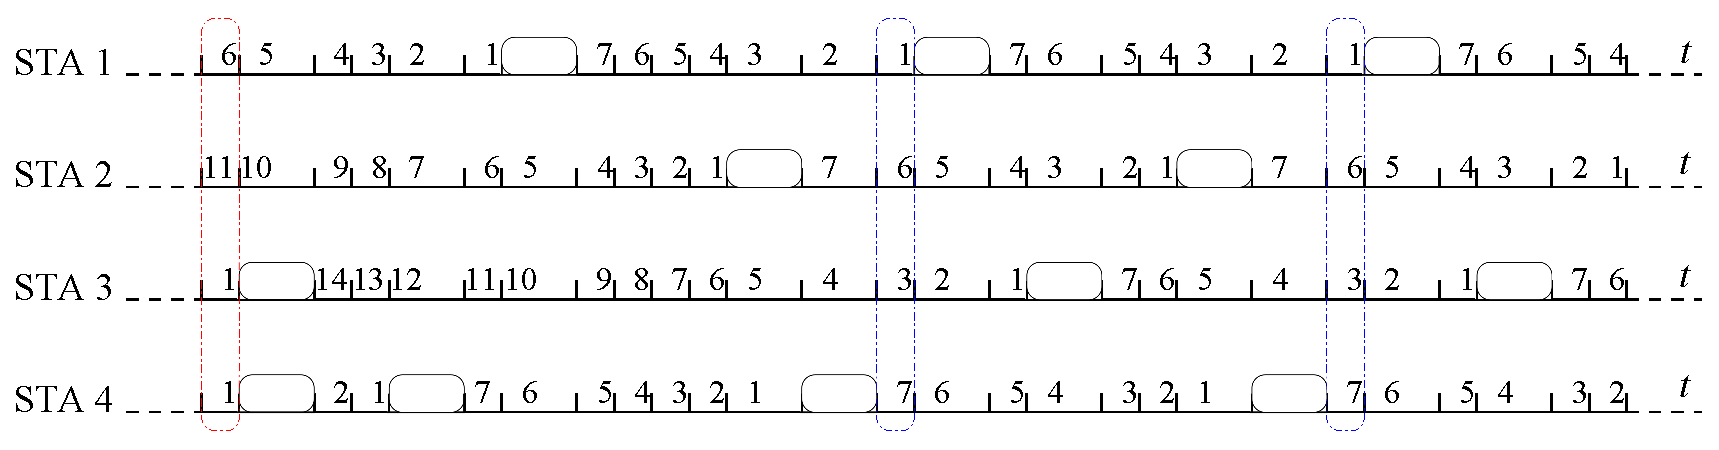
\includegraphics[width=0.8\linewidth]{figures/basicECA.eps}
  \caption{CSMA/ECA example in saturation}
  \label{fig:BECA}
\end{figure*}

In Figure~\ref{fig:BECA}, the \emph{STA~\#} labels represent stations willing to transmit. The horizontal lines are a time abstraction with each number indicating the amount of empty slots left for the backoff to expire. Stations willing to transmit begin the contention for the channel by picking a random backoff, $B$. The red outline highlights the fact that stations STA 3 and STA 4 will eventually collide because they selected the same $B$. After recomputing the random backoff, STA 4's attempt results in a successful transmission, which instructs the node to pick a deterministic backoff, $B_{d}=7$ in this case. By doing so, all successful STAs will not collide among each other in future cycles.

Collision slots being orders of magnitude larger than empty slots degrade the network performance. When CSMA/ECA builds the collision-free schedule all contenders are able to successfully transmit more often, increasing the aggregated throughput beyond DCF's. Figure~\ref{fig:BECA-throughput} shows the achieved throughput of CSMA/ECA and CSMA/CA, alongside the Jain's Fairness Index (JFI)~\cite{JFI}.

\begin{figure}[htbp]
\centering
  \includegraphics[width=0.7\linewidth, angle=-90]{figures/DCF-vs-ECA.eps}
  \caption{CSMA/ECA example in saturation}
  \label{fig:BECA}
\end{figure}

Referring to Figure~\ref{fig:BECA}, CSMA/ECA is able to achieve an aggregated throughput that goes beyond CSMA/CA up until the number of contenders ($N$) is greater than $B_{d}=7$. Beyond this point, the network will have a mixed behavior relating to backoff mechanism: some nodes will successfully transmit and pick a deterministic backoff while others will collide due to the lack of empty slots and return to a random backoff. As more contenders join the network, CSMA/ECA performance will approximate to CSMA/CA's.

The \emph{JFI for CSMA/ECA} and \emph{JFI for CSMA/CA} curves in Figure~\ref{fig:BECA} show the Jain's Fairness index for both protocols. A value equal to one throughout the range of contenders suggests that the available throughput is shared evenly among all stations.

	\subsection{Supporting many more contenders}
	As was mentioned before, CSMA/ECA is only able to build a collision-free schedule if the number of contenders $N$, is less or equal than $B_{d}$. When $N > B_{d}$, collisions reappear. 
	
	To recover the collision-free schedule, CSMA/ECA instructs nodes {\bfseries not} to reset their backoff stage ($k$) after successful transmissions, but to pick a deterministic backoff $B_{d}=CW(k)/2$; where $CW(k)=2^{k}CW_{\min}$. This measure allocates many more contenders in a collision-free schedule and is called \emph{Hysteresis}.
	
	Hysteresis enables CSMA/ECA nodes to have different schedules ($B_{d}$), carrying the undesired effect of unevenly divide the channel time among contenders (some nodes will have to wait more in order to attempt transmissions).
	
	This unfairness is leveraged by instructing nodes at backoff stage $k$ to transmit $2^{k}$ packets on each attempt, thus proportionally compensating those nodes at higher backoff stages. This measure was first proposed by Fang. et al. in~\cite{L_MAC}, and further implemented as \emph{Fair Share} for CSMA/ECA~\cite{research2standards}. Figure~\ref{fig:fairness} shows the JFI for CSMA/CA as well as for CSMA/ECA with both enhancements: Hysteresis and Fair Share.
	
	\begin{figure}[htbp]
	\centering
		\includegraphics[width=0.7\linewidth, angle=-90]{figures/fairness-combined.eps}
		\caption{Fairness comparison with nodes under saturation}
		\label{fig:fairness}
	\end{figure}
	
	In Figure~\ref{fig:fairness}, the only curve deviating from JFI = 1 is \emph{CSMA/ECA w/ hysteresis}; suggesting an uneven partition of the channel access time among contenders.
	
	\begin{figure*}[tbhp]
	\centering
		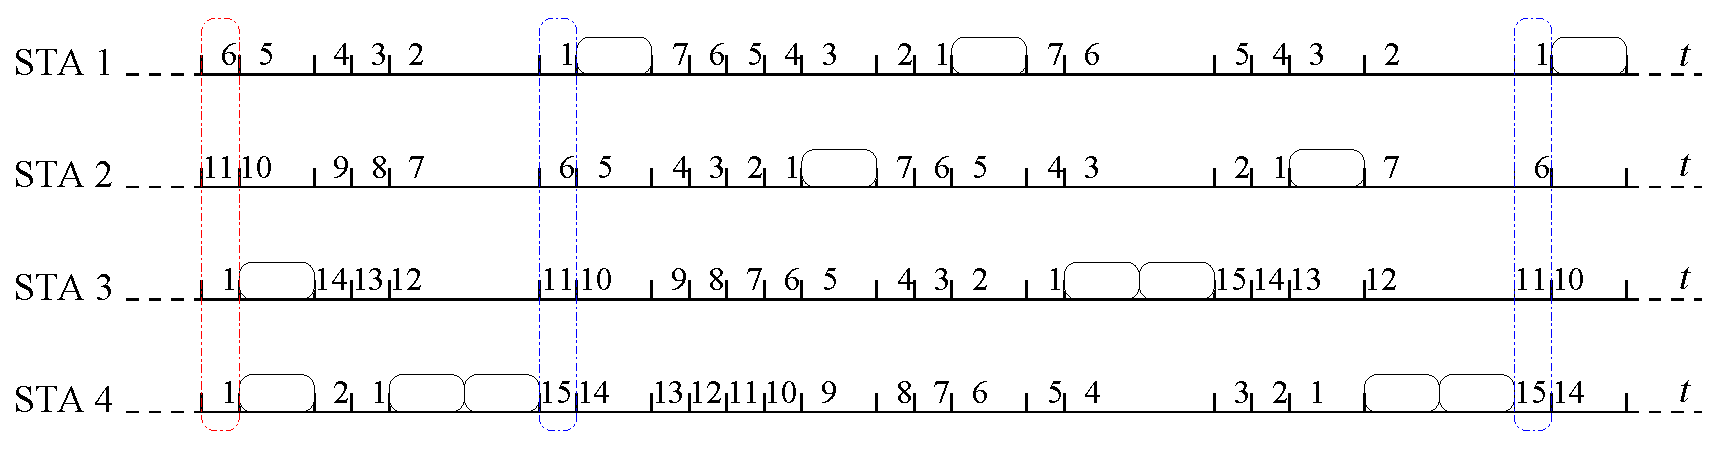
\includegraphics[width=0.8\linewidth]{figures/csma_eca_different_backoff_short.eps}
		\caption{CSMA/ECA + Hysteresis example in saturation ($CW_{\min}=16$)}
		\label{fig:ECA+Hyst}
	\end{figure*}
	
	As with Figure~\ref{fig:BECA}, Figure~\ref{fig:ECA+Hyst} shows four stations attempting to transmit. The red outline indicates a collision between STA 3 and STA 4, which will provoke an increment on both station's backoff stage ($k=k+1$). Once STA 4's random backoff expires, CSMA/ECA instructs the station to transmit $2^{k}$ packets, and then pick a deterministic backoff, $B_{d}=CW(k)/2$. The same behavior is followed by STA 3.
	
	With Hysteresis and Fair Share, CSMA/ECA is able to achieve greater throughput than CSMA/CA and for many more contenders, as shown in Figure~\ref{fig:ECA+H+F-throughput} extracted from~\cite{research2standards}. In the figure, the \emph{CSMA/ECA with Hysteresis and Fair Share} curve shows a greater throughput because collisions are eliminated and Fair Share allows nodes to send $2^{k}$ packets upon each transmission.

	\begin{figure}[htbp]
	\centering
		\includegraphics[width=0.7\linewidth,angle=-90]{figures/throughput-combined.eps}
		\caption{Throughput comparison~\cite{research2standards}}
		\label{fig:ECA+H+F-throughput}
	\end{figure}
	
	\subsection{Endurance to clock drift}
	
	
	
\section{Simulation}\label{simulations}
\section{Prototyping CSMA/ECA}\label{prototype}
\section{Coexistence with CSMA/CA}\label{prototypeResults}
\section{Conclusions}\label{conclusions}
\section{Acknowledgements}


\bibliographystyle{IEEEtran}
\bibliography{../ref}

\end{document}